\documentclass{article}
\usepackage[T1]{fontenc}
\usepackage[utf8]{inputenc}
\usepackage{amsmath, amssymb}
\usepackage{babel}
\usepackage{fullpage}
\usepackage{hyperref,url}
\usepackage{tcolorbox}
\usepackage{booktabs}
\usepackage{siunitx}
\usepackage{threeparttable}
\usepackage{float}
\usepackage{graphicx}

\sisetup{
  detect-all,
  output-exponent-marker = \mathrm{e},
  table-number-alignment = center
}

\providecommand{\e}[1]{\ensuremath{\times 10^{#1}}}
\setlength{\parindent}{0pt}

\title{Answers to Empirical IO I: Problem Set 2}
\author{}
\date{}

\begin{document}
\maketitle

\begin{tcolorbox}
You will estimate demand and supply in a stylized model of the market for
pay-TV services. You will use any programming language (Python/R/Matlab/Julia) to create your own fake data set for the industry and do some
relatively simple estimation. Then, using the \texttt{pyBLP} package of Conlon and Gortmaker, you will
estimate the model and perform some merger simulations.\footnote{%
Using data you generate yourself gives you a way to check whether the
estimation is working; this is a good thing to try whenever you code up an
estimator!}. The pyBLP package has excellent
documentation and a very helpful tutorial (which covers merger simulation),
both easy to find (\url{https://pyblp.readthedocs.io/en/stable/}). You may want to work through the tutorial notebooks available with the documentation (or on the Github page).\\

To install \texttt{pyBLP} you need to have Python 3 installed, I recommend Anaconda \url{https://www.anaconda.com/distribution/}. If you have python installed you simply need to type:
\begin{verbatim}
pip install pyblp
\end{verbatim}
or 
\begin{verbatim}
pip install git+https://github.com/jeffgortmaker/pyblp
\end{verbatim}

Please submit a \underline{single printed} document presenting your answers to the questions below,
requested results, and code. Write this up cleanly with nice tables where appropriate.
You may work in groups of up to 3 on the coding, but your write-up must be your own work and must indicate who your partners are.

You can do parts (2) and (3) in R, Matlab, Julia, or Python. Parts (4) and (5) use \texttt{pyblp} which you can run in R using \texttt{reticulate} if you really want.
\end{tcolorbox}

\begin{tcolorbox}
There are $T$ markets, each with four inside goods $j\in
\{1,2,3,4\}$ and an outside option. Goods 1 and 2 are satellite television
services (e.g., DirecTV and Dish); goods 3 and 4 are wired television
services (e.g., Frontier and Comcast in New Haven).
The conditional indirect utility of consumer $i$ for good $j$ in market $t$
is given by
\begin{align*}
u_{ijt}& =\beta ^{\left( 1\right) }x_{jt}+\beta
_{i}^{(2)}satellite_{jt}+\beta _{i}^{(3)}wired_{jt}+\alpha p_{jt}+\xi
_{jt}+\epsilon _{ijt}\text{ \qquad }j>0 \\
u_{i0t}& =\epsilon _{i0t},
\end{align*}%
where $x_{jt}$ is a measure of good $j$'s quality, $p_{jt}$ is its price, $%
satellite_{jt}$ is an indicator equal to 1 for the two satellite services,
and $wired_{jt}$ is an indicator equal to 1 for the two wired services. The
remaining notation is as usual in the class notes, including the i.i.d.
type-1 extreme value $\epsilon _{ijt}$.  Each consumer purchases the good giving them the highest conditional indirect utility.

Goods are produced by single-product firms. Firm $j$'s (log) marginal
cost in market $t$ is 
\begin{equation*}
\ln mc_{jt}=\gamma ^{0}+\text{w}_{jt}\gamma ^{1}+\omega _{jt}/8,
\end{equation*}%
where w$_{jt}$ is an observed cost shifter. Firms compete by simultaneously choosing prices in each market under complete information. Firm $j$ has profit
\begin{equation*}
\pi _{jt}=\max_{p_{jt}}M_{t}(p_{jt}-mc_{jt})s_{jt}(p_{t}).
\end{equation*}
\end{tcolorbox}

% ----------------------------- Generate Fake Data -----------------------------
\section*{Generate Fake Data}

\begin{tcolorbox}
\textbf{1.} Draw the exogenous product characteristic $x_{jt}$ for $T=600$
geographically defined markets (e.g., cities). Assume each $x_{jt}$ is equal
to the absolute value of an iid standard normal draw, as is each w$_{jt}$.
Simulate demand and cost unobservables as well, specifying
\begin{equation*}
\left(
\begin{array}{c}
\xi _{jt} \\
\omega _{jt}%
\end{array}%
\right) \sim N\left( \left(
\begin{array}{c}
0 \\
0%
\end{array}%
\right) ,\left(
\begin{array}{cc}
1 & 0.25 \\
0.25 & 1%
\end{array}%
\right) \right) \text{ iid across }j,t.
\end{equation*}

Let
\begin{eqnarray*}
\beta ^{(1)} &=&1\text{, }\beta _{i}^{\left( k\right) }\sim \text{iid }%
N\left( 4,1\right) \text{ for }k=2,3 \\
\alpha  &=&-2 \\
\gamma ^{(0)} &=&1/2\text{, }\gamma ^{(1)}=1/4.
\end{eqnarray*}
\end{tcolorbox}

\textbf{1.} See Julia code.

\begin{tcolorbox}
\textbf{2(a).} Start by writing a procedure to approximate the derivatives of market
shares with respect to prices (taking prices, shares, $x$, and demand
parameters as inputs). The key steps are:
\begin{enumerate}
\item For each $(j,t)$, write the choice probability $s_{jt}$ as a weighted
average (integral) of the (multinomial logit) choice probabilities
conditional on the value of each consumer's random coefficients;
\item Anticipating differentiation under the integral sign, derive the
analytical expression for the derivative of the \textit{integrand} with
respect to each $p_{kt}$; 
\item Use the expression you obtained in (2) and simulation draws of the
random coefficients to approximate the integral that corresponds to $%
\partial s_{jt}/\partial p_{kt}$ for each $j$ and $k$ (i.e., replace
the integral with the mean over the values at each simulation draw).
\item Experiment to see how many simulation draws you need to get precise
approximations and check this again at the equilibrium shares and prices you
obtain below. \newline
\end{enumerate}
Note: you do not want to take new simulation draws of the random
coefficients each time you call this procedure. This is because,  if you did so, the attempt
to solve for equilibrium prices (below) may never converge due to \textquotedblleft
jittering\textquotedblright\ across iterations. So take your simulation draws only once, outside the procedure you write here. 
\end{tcolorbox}
\textbf{2(a).}

I've summarised the analytic parts of the steps below alongside implementing them in the code.

\paragraph{Step 1:}

For a consumer with random coefficients $b=(\beta^{(2)},\beta^{(3)})$ in market $t$, the deterministic utility for $j>0$ is
\[
V_{jt}(b) \;=\; \beta^{(1)} x_{jt} \;+\; \alpha p_{jt} \;+\; \xi_{jt}
\;+\; \beta^{(2)} \,\text{satellite}_{jt} \;+\; \beta^{(3)} \,\text{wired}_{jt},
\qquad V_{0t}(b) = 0.
\]
Conditional choice probabilities for this consumer are
\[
s_{jt}(p\,|\,b) \;=\; \frac{\exp\!\big(V_{jt}(b)\big)}{1 + \sum_{\ell=1}^J \exp\!\big(V_{\ell t}(b)\big)}
\quad\text{for } j=1,\dots,J,
\qquad
s_{0t}(p\,|\,b) \;=\; \frac{1}{1 + \sum_{\ell=1}^J \exp\!\big(V_{\ell t}(b)\big)}.
\]
Let $F$ denote the distribution of $b$. Market shares are the integral of conditional probabilities:
\[
s_{jt}(p) \;=\; \int s_{jt}(p\,|\,b)\, dF(b), \qquad j=0,1,\dots,J.
\]

Where here $F$ is such that $\beta^{(k)}\sim N(4,1)$ i.i.d.\ for $k=2,3$.

\vspace{5mm}

These conditional shares are calculated in conditional\_shares\_matrix() in code.


\paragraph{Step 2}
For $k\in\{1,\dots,J\}$, note that $\partial V_{\ell t}(b) / \partial p_{kt} = \alpha\,\mathbf{1}\{\ell=k\}$.
The logit derivative identity gives, for each fixed $b$,
\[
\frac{\partial s_{jt}(p\,|\,b)}{\partial p_{kt}}
\;=\;
\alpha\, s_{jt}(p\,|\,b)\,\big(\mathbf{1}\{j=k\} - s_{kt}(p\,|\,b)\big).
\]
Equivalently, in matrix form for the inside good vector $s_t(p\,|\,b)\in\mathbb{R}^J$,
\[
\frac{\partial s_t(p\,|\,b)}{\partial p_t}
\;=\;
\alpha\,\Big(\mathrm{Diag}\big(s_t(p\,|\,b)\big) - s_t(p\,|\,b)\,s_t(p\,|\,b)^\top\Big).
\]
i.e. own-price effects on the diagonal and cross-price off it.

\paragraph{Step 3}
Let $\{b^{(m)}\}_{m=1}^M$ be simulation draws from $F$. Then
\[
\frac{\partial s_{jt}(p)}{\partial p_{kt}}
\;=\;
\int \alpha\, s_{jt}(p\,|\,b)\,\big(\mathbf{1}\{j=k\} - s_{kt}(p\,|\,b)\big)\, dF(b)
\;\approx\;
\frac{1}{M}\sum_{m=1}^M \alpha\, s_{jt}\big(p\,|\,b^{(m)}\big)\,\big(\mathbf{1}\{j=k\} - s_{kt}\big(p\,|\,b^{(m)}\big)\big).
\]
In matrix form,
\[
\frac{\partial s_t(p)}{\partial p_t}
\;\approx\;
\alpha\,\frac{1}{M}\sum_{m=1}^M
\Big(\mathrm{Diag}\big(s_t(p\,|\,b^{(m)})\big) - s_t(p\,|\,b^{(m)})\,s_t(p\,|\,b^{(m)})^\top\Big).
\]

\vspace{5mm}

jacobian\_dsdp\_market() implements this in the code.

\paragraph{Step 4:} The average derivative values (under random prices) seem to level out once the number of draws hits around 500.

\begin{figure}[H]
    \centering
    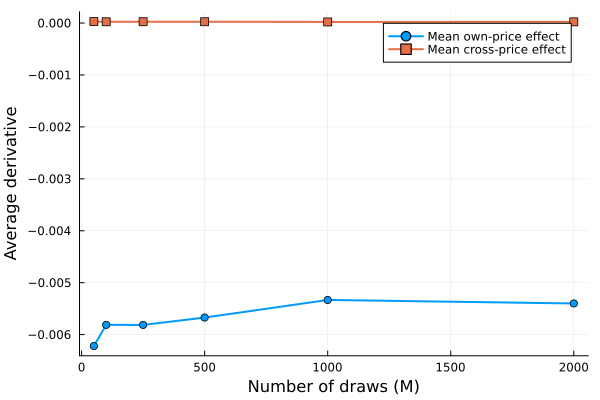
\includegraphics[width=0.7\textwidth]{experiment_draws_convergence_random_prices.png}
    \caption{Convergence of simulated Jacobian elements as the number of random coefficient draws $M$ increases.}
    \label{fig:draws_convergence}
\end{figure}

\begin{tcolorbox}
\textbf{2(b).} The FOC for firm $j$'s profit maximization problem in market $t$ is
\begin{align}
(p_{jt}-mc_{jt})\frac{\partial s_{jt}(p_{t})}{\partial p_{jt}}+s_{jt}& =0
\notag \\
\implies p_{jt}-mc_{jt}& =-\left( \frac{\partial s_{jt}(p_{t})}{\partial
p_{jt}}\right) ^{-1}s_{jt}  \label{FOC}
\end{align}
\end{tcolorbox}

\begin{tcolorbox}
\textbf{2(c).} Substituting in your approximation of each $\left( \frac{\partial
s_{jt}(p_{t})}{\partial p_{jt}}\right) $, solve the system of equations (\ref%
{FOC}) ($J\,$equations per market) for the equilibrium prices in each market.

\begin{enumerate}
\item To do this you will need to solve a system of $J \times J$ nonlinear equations.\footnote{To do this in Python use \texttt{scipy.optimize.root}, in MATLAB use \texttt{fsolve}, in R use \texttt{nleqslv} or something similar, and in Julia use \texttt{NLSolve.jl} or something similar.} Make sure to check the exit flag for each market to make sure you have a solution. 
\item Do this again using the algorithm of Morrow and
Skerlos (2011), discussed in section 3.6 of Conlon and Gortmaker (2019) (and
in the \texttt{pyBLP} \textquotedblleft problem simulation tutorial\textquotedblright
). Use the numerical integration approach you used in step (a) to approximate the
terms defined in equation (25) of Conlon and Gortmaker. If you get different
results using this method, resolve this discrepancy either by correcting
your code or explaining why your preferred method is the one to be trusted.
\end{enumerate}
\end{tcolorbox}

See Julia code - solved with both methods and had max $|\Delta p|$ across markets = 3.84e-8

\begin{tcolorbox}
\textbf{3.} Calculate \textquotedblleft observed\textquotedblright\ shares for
your fake data set using your parameters, your draws of $x,$w$,\beta
_{i},\omega ,\xi $, and your equilibrium prices.
\end{tcolorbox}

See Julia code. Example plot using these shares (aggregating the goods by their characteristic) below:

\begin{figure}[H]
  \centering
  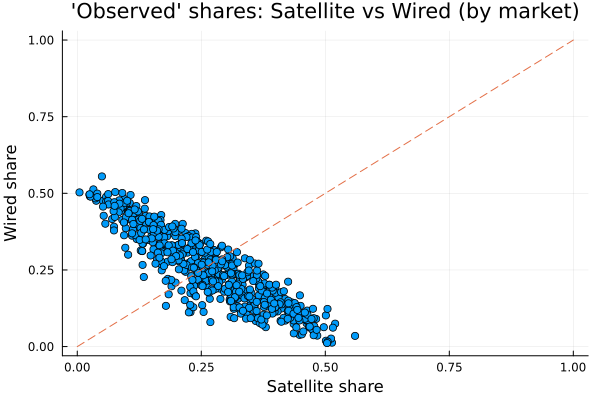
\includegraphics[width=0.8\textwidth]{q3_sat_vs_wired.png}
  \caption{Observed shares for each type of TV at equilibrium across $T=600$ markets}
  \label{fig:q3_shares}
\end{figure}


% ----------------------------- Mis-specified Models -----------------------------
\section*{Estimate Some Mis-specified Models}

\begin{tcolorbox}
\textbf{4.} Estimate the plain multinomial logit model of demand by OLS\
(ignoring the endogeneity of prices).
\end{tcolorbox}

\paragraph{4.} Let $y_{jt}=\ln s_{jt}-\ln s_{0t}$. (i.e. the Berry inversion) The plain logit implies
\[
y_{jt}= \beta x_{jt} + \alpha p_{jt} + \xi_{jt},
\]
which we estimate by OLS, ignoring the endogeneity of $p_{jt}$.

\begin{tcolorbox}
\textbf{5.} Re-estimate the multinomial logit model of demand by two-stage
least squares, instrumenting for prices with the exogenous demand shifters $%
x $ and excluded cost shifters w. Discuss how the results differ from those
obtained by OLS.
\end{tcolorbox}

\textbf{5.} Let the first stage be $p_{jt}=\pi_0+\pi_1 x_{jt}+\pi_2 w_{jt}+u_{jt}$.
The 2SLS second stage is
\[
y_{jt}= \beta x_{jt} + \alpha \hat p_{jt} + \varepsilon_{jt},
\]
instrumenting price with $\{x_{jt},w_{jt}\}$.

\begin{table}[H]
\centering
\caption{Plain logit estimates: OLS vs 2SLS (instrumenting price with x and w).}
\begin{tabular}{lccc}
\toprule
Parameter & OLS & 2SLS & True\\
\midrule
Beta on x & 0.779 & 1.136 & 1.0\\
Beta on satellite & 0.153 & 0.473 & --\\
Alpha on price & -0.782 & -0.972 & -2.0\\
\bottomrule
\end{tabular}
\end{table}


The OLS estimate of the price coefficient is less negative than the 2SLS estimate. This is unsurprising given price endoegneity in equilibrium: firms set higher prices in markets with positive demand shocks~($\xi_{jt}$). OLS confounds movements along the demand curve with shifts in demand, tracing out a weighed mixture of supply and demand rather than the true demand curve. Instrumenting price with exogenous shifters~($x_{jt}$ and $w_{jt}$) isolates variation in price that is uncorrelated with~$\xi_{jt}$, yielding a steeper estimate.

\vspace{5mm}

Still, the 2SLS is misspecified and is a magnitude off the true $\alpha$ estimate. Even with valid instruments and infinite data, 2SLS converges to the wrong slope $\alpha^\ast$ for the misspecified model, not to the structural $\alpha=-2$. Second, instrument strength is limited here: the excluded cost shifter $w_{jt}$ moves prices only modestly ($\gamma^{(1)}=\tfrac{1}{4}$) and there is simultaneity from $\mathrm{corr}(\xi,\omega)=0.25$, so the first stage is weak and finite–sample bias pulls $\hat\alpha^{2SLS}$ back toward OLS. Third, technology effects (satellite/wired) and their heterogeneity will go into the error if not controlled, creating residual correlation between price and the error even after instrumenting. Together these imply $\hat\alpha^{2SLS}\to \alpha^\ast\neq -2$, explaining why the IV estimate is more negative than OLS but still far from the true parameter.








\begin{tcolorbox}
\textbf{6.} Now estimate a nested logit model by two-stage least squares,
treating \textquotedblleft satellite\textquotedblright\ and
\textquotedblleft wired\textquotedblright\ as the two nests for the inside
goods. You will probably want to review the discussion of the nested logit
in Berry (1994). Note that Berry focuses on the special case in which all
the \textquotedblleft nesting parameters\textquotedblright\ are the same;
you should allow a different nesting parameter for each nest.\footnote{%
In Berry's notation, this means letting the parameter $\sigma $ become $%
\sigma _{g(j)}$, where $g\left( j\right) $ indicates the group (satellite or
wired) to which each inside good $j$ belongs.} Without reference to the
results, explain the way(s) that this model is misspecified. (Hint: students
tend to get this question wrong; recall that I suggested you review Berry
94).
\end{tcolorbox}

\begin{table}[H]
\centering
\caption{Nested logit estimates (2SLS).}
\begin{tabular}{lc}
\toprule
Parameter & Estimate\\
\midrule
Beta on $x$ & 0.915\\
Alpha on price & -0.753\\
Sigma (satellite) & 3.046\\
Sigma (wired) & -2.649\\
\bottomrule
\end{tabular}
\end{table}


The nested logit model is misspecified because it imposes a mechanical pattern of correlation in unobserved utility within the predefined nests rather than modeling true taste heterogeneity. As Berry (1994) notes, the nested logit allows substitution patterns to depend only on group membership and not on continuous characteristics of products or consumers. In the true random coefficients model, substitution depends on how similar products are in characteristics and on heterogeneous consumer tastes. By restricting correlation to fixed nests, the nested logit cannot capture these richer substitution patterns and will therefore misstate cross-price elasticities and substitution across technologies.

\vspace{5mm}

It's interesting that its estimates are even further from the true parameters than even plain OLS. The conditional share terms are built from market shares so inherit dependence on the demand shock $\xi_{jt}$. When we treat it as exogenous, its bias spills into the price coefficient and might attentuate $\hat\alpha$ more than even in plain OLS or 2SLS. Similarly, the fact we use a finite sample might mean measurement error on the conditional shares which further attenuates the estimates.


\begin{tcolorbox}
\textbf{7.} Using the nested logit results, provide a table comparing the
estimated own-price elasticities to the true own-price elasticities.% 
\footnote{%
The procedure you developed above for approximating derivatives cannot be
used for your estimates based on the nested logit model. But because we have
analytic expressions for market shares in the nested logit model, you could
either differentiate these or use \textquotedblleft finite
difference\textquotedblright\ approximation of derivatives.} Provide two
additional tables showing the true matrix of diversion ratios and the
diversion ratios implied by your estimates.\footnote{If you get stuck working out the diversion ratios for nested logit -- consult Conlon and Mortimer (2018).}
\end{tcolorbox}

\begin{table}[H]
\centering
\caption{Average own-price elasticities across markets.}
\begin{tabular}{lcc}
\hline
Product & True & Nested logit est.\\
\hline
Good 1 & -5.317 & -3.189\\
Good 2 & -5.262 & -3.046\\
Good 3 & -5.268 & -3.316\\
Good 4 & -5.308 & -3.476\\
\hline
\end{tabular}
\end{table}

\begin{table}[H]
\centering
\caption{Average diversion ratios across markets (true).}
\begin{tabular}{lcccc}
\hline
From\\To & 1 & 2 & 3 & 4\\
\hline
1 & -1.000 & 0.205 & 0.123 & 0.119\\
2 & 0.196 & -1.000 & 0.123 & 0.120\\
3 & 0.124 & 0.131 & -1.000 & 0.186\\
4 & 0.122 & 0.129 & 0.193 & -1.000\\
\hline
\end{tabular}
\end{table}

\begin{table}[H]
\centering
\caption{Average diversion ratios across markets (nested-logit estimate).}
\begin{tabular}{lcccc}
\hline
From\\To & 1 & 2 & 3 & 4\\
\hline
1 & -1.000 & 0.535 & 0.075 & 0.069\\
2 & 0.510 & -1.000 & 0.077 & 0.075\\
3 & 0.071 & 0.075 & -1.000 & 0.533\\
4 & 0.066 & 0.074 & 0.554 & -1.000\\
\hline
\end{tabular}
\end{table}



% ----------------------------- Correct Model with pyBLP -----------------------------
\section*{Estimate the Correctly Specified Model}

\begin{tcolorbox}
\textbf{8.} Report a table with the estimates of the demand
parameters and standard errors. Do this three times: once when you estimate demand
alone, then again when you estimate jointly with supply; and again with the ``optimal IV''.
\end{tcolorbox}

Since the satellite and wired dummies partition all the inside goods, we can't just identify the random coefficients on them both. Intuitively, we could never separate an observed relative preference for satellite over wired into how much the consumer likes about satellite TV vs dislikes about wired TV from the aggregate data on market shares. We would need extra moments for the GMM (like microdata) to provide the extra restrictions to unpack this.

\vspace{5mm}

Therefore here, it's sufficient to move to a single random coefficient on satellite and include an intercept in mean utility, dropping the other dummy from the means. In this parameterisation, the random part is
\[
(\beta_i^{satellite} - \beta_i^{wired}) \cdot \text{satellite}_j,
\]
and the consumer-specific intercept $\beta_i^{wired}$ is absorbed by the mean intercept. The identified heterogeneity is therefore the difference $(\beta_i^{sat} - \beta_i^{wir})$.

\vspace{5mm}

Note that this coefficient should have a ``true'' mean of zero and an SD of $\sqrt{2} \approx 1.414$, since under the DGP $\beta_i^{satellite}$ and $\beta_i^{wired}$ were drawn independently from $\mathcal{N}(4,1)$.

\vspace{5mm}

We need quite a few instruments to get the number of moments above the number of parameters and identify the model. I combined the exogenous product characteristics and cost shifters with BLP-style constructed variables: the exogenous shifters $x_{jt}$, $w_{jt}$, the dummies satellite and wired, the sum of rival product characteristics within each market, the BLP differentiation instruments based on $x$, and the same-nest quality index (the sum of $x$ among other products of the same technology within the market).  The supply side is instrumented using $x_{jt}$ as the excluded shifter in the marginal cost equation.


\begin{table}[H]
\centering
\caption{Random-coefficients logit estimates (PyBLP). Entries are estimate (s.e.).}
\begin{tabular}{lccc}
\hline
Parameter & Demand only & Demand+Supply & Optimal IV\\
\hline
$\beta_x$ & 0.801 (0.042) & 0.800 (0.042) & 0.781 (0.032)\\
$\alpha_{price}$ & -1.889 (0.085) & -1.889 (0.085) & -1.874 (0.067)\\
Mean on satellite & -0.234 (0.202) & -0.234 (0.201) & 0.079 (0.055)\\
SD on satellite & 1.372 (0.443) & 1.370 (0.443) & 0.455 (0.212)\\
\hline
\end{tabular}
\end{table}



The smaller estimated standard deviation in the optimal IV spec could reflect collinearity among the generated optimal instruments, since the optimal-IV step produces instrument functions that are nearly linear combinations of existing ones. The weighting matrix then down weights the moments that help identify the dispersion and pulls $\hat{\sigma}$ toward smaller values.





\begin{tcolorbox}
\textbf{9.} Using your preferred estimates from the prior step (explain your
preference), provide a table comparing the estimated own-price elasticities
to the true own-price elasticities. Provide two additional tables showing
the true matrix of diversion ratios and the diversion ratios implied by your
estimates.
\end{tcolorbox}

I chose the demand+supply spec above, given the potential collinearity issue with the optimal IV. 

\begin{table}[H]
\centering
\caption{Average own-price elasticities (true vs estimated).}
\begin{tabular}{lcc}
\hline
Product & True & Estimated\\
\hline
$1$ & -5.317 & -4.801\\
$2$ & -5.262 & -4.734\\
$3$ & -5.268 & -5.153\\
$4$ & -5.308 & -5.177\\
\hline\end{tabular}\end{table}

\begin{table}[H]\centering
\caption{Average diversion ratios across markets (true).}
\begin{tabular}{lcccc}\hline From\\To & 1 & 2 & 3 & 4\\\hline
1 & -1.000 & 0.205 & 0.123 & 0.119\\
2 & 0.196 & -1.000 & 0.123 & 0.120\\
3 & 0.124 & 0.131 & -1.000 & 0.186\\
4 & 0.122 & 0.129 & 0.193 & -1.000\\
\hline\end{tabular}\end{table}

\begin{table}[H]\centering
\caption{Average diversion ratios across markets (estimated).}
\begin{tabular}{lcccc}\hline From\\To & 1 & 2 & 3 & 4\\\hline
1 & -1.000 & 0.261 & 0.130 & 0.125\\
2 & 0.249 & -1.000 & 0.131 & 0.127\\
3 & 0.114 & 0.120 & -1.000 & 0.151\\
4 & 0.112 & 0.119 & 0.155 & -1.000\\
\hline\end{tabular}\end{table}


% ----------------------------- Merger Simulation -----------------------------
\section*{Merger Simulation}

\begin{tcolorbox}
\textbf{10.} Suppose two of the four firms were to merge. Give a brief
intuition for what theory tells us is likely to happen to the equilibrium
prices of each good $j$.
\end{tcolorbox}

When two firms merge, they internalise diversion between their products. The FOCs add markups on each product proportional to the diversion to the merged partner. Own prices of the merging products rise the most; non-merging rivals also tend to increase prices because higher prices on the merged products soften competition. The magnitude should depend on the relative strength of diversion within and on price sensitivity.

\begin{tcolorbox}
\textbf{11.} Suppose firms 1 and 2 are proposing to merge. Use the \texttt{pyBLP}
merger simulation procedure to provide a prediction of the post-merger
equilibrium prices.
\end{tcolorbox}

See Julia code.

\begin{tcolorbox}
\textbf{12.} Now suppose instead that firms 1 and 3 are the ones to merge.
Re-run the merger simulation. Provide a table comparing the (average
across markets) predicted merger-induced price changes for this merger and
that in part 11. Interpret the differences between the predictions for the
two mergers.
\end{tcolorbox}

\begin{table}[H]
\centering
\caption{Average post-merger prices by product: merger of firms 1 \& 2}
\begin{tabular}{lcc}
\hline Product & Pre-merger & Post-merger \\ \hline
$1$ & 3.177 & 3.387 \\
$2$ & 3.182 & 3.379 \\
$3$ & 3.154 & 3.156 \\
$4$ & 3.150 & 3.152 \\
\hline\end{tabular}\end{table}

\begin{table}[H]
\centering
\caption{Average post-merger prices by product: merger of firms 1 \& 3}
\begin{tabular}{lcc}
\hline Product & Pre-merger & Post-merger \\ \hline
$1$ & 3.177 & 3.256 \\
$2$ & 3.182 & 3.186 \\
$3$ & 3.154 & 3.237 \\
$4$ & 3.150 & 3.151 \\
\hline\end{tabular}\end{table}

\begin{table}[H]
\centering
\caption{Average price changes (post $-$ pre) by product and difference}
\begin{tabular}{lccc}
\hline Product & Merger 1--2 & Merger 1--3 & Difference \\ \hline
$1$ & 0.210 & 0.078 & 0.132 \\
$2$ & 0.198 & 0.005 & 0.193 \\
$3$ & 0.002 & 0.083 & -0.081 \\
$4$ & 0.002 & 0.001 & 0.001 \\
\hline\end{tabular}\end{table}


Since 1 and 2 are closer substitutes (as satellite services), the price effects are stronger for good 1 when it merges with 2, as compared to when it merges with 3. It's not immediately obvious why there is a negative price effect for product 3 under the mergers, but perhaps they happen to have higher simulated marginal costs than 1 or much smaller initial shares (they raise the price of 1 to extract surplus from price inelastic consumers of 1 but reduce the price of 3 to ensure the diverted more elastic customers go to 3). This is possible because of the nonlinearity of the price system.


\begin{tcolorbox}
\textbf{13.} Thus far you have assumed that there are no \textquotedblleft
efficiencies\textquotedblright\ (reduction in costs) resulting from the
merger. Explain briefly why a merger-specific reduction in marginal cost
could mean that a merger is welfare-enhancing.
\end{tcolorbox}

A merger led cost reduction shifts post-merger pricing tradeoffs: lower costs reduce the optimal markups needed to satisfy FOCs and directly lower deadweight loss. If the cost savings are sufficiently large, consumer surplus can rise and total welfare can improve even if some prices still increase.


\begin{tcolorbox}
\textbf{14.} Consider the merger between firms 1 and 2, and suppose the firms
demonstrate that by merging they would reduce marginal cost of each of their
products by 15\%. Furthermore, suppose that they demonstrate that this cost
reduction could not be achieved without merging.    Using the \texttt{pyBLP} software, re-run the merger simulation
with the 15\% cost saving. Show the predicted post-merger price changes (again,
for each product, averaged across markets). What is the predicted impact of
the merger on consumer welfare,\footnote{%
Note that because we have quasilinear preferences, consumer surplus is a
valid measure of aggregate consumer welfare under the usual assumption of
optimal redistribution.} assuming that the total measure of consumers $%
M_{t} $ is the same in each market  $t$?  
\end{tcolorbox}

\begin{table}[H]
\centering
\caption{Merger 1--2 with 15\% cost reduction: average price changes by product}
\begin{tabular}{lc}
\hline Product & $\Delta p$ \\ \hline
$1$ & -0.060 \\
$2$ & -0.071 \\
$3$ & -0.003 \\
$4$ & -0.003 \\
\hline\end{tabular}\end{table}



\begin{table}[H]
\centering
\caption{Average change in consumer surplus (per consumer)}
\begin{tabular}{lc}
\hline $\Delta CS$ & 0.033 \\ \hline
\end{tabular}\end{table}



\begin{tcolorbox}
\textbf{15.} Explain why this additional assumption
(or data on the correct values of $M_{t}$) is needed here, whereas up to
this point it was without loss to assume $M_{t}=1$. What is the predicted
impact of the merger on total welfare?
\end{tcolorbox}

Up to now, normalising $M_t=1$ was without loss for estimation and price/comparison tables because everything scaled out. Consumer surplus and producer surplus scale linearly with $M_t$: $CS_t = M_t \cdot cs_t$ and $\Pi_t = M_t \cdot \sum_j (p_{jt}-mc_{jt}) s_{jt}$. To aggregate welfare levels across markets, we need the actual $M_t$. Total welfare change equals the change in consumer surplus plus the change in producer surplus; both require $M_t$ for impacts in levels.

\section*{Coding Tips}
\begin{tcolorbox}
\begin{itemize}
 \item You can draw from a multivariate normal with variance $\Sigma $ by
drawing independent standard normal random variables and using the Cholesky
decomposition of $\Sigma $ (the latter obtained with \texttt{chol} in Matlab or \texttt{numpy.linalg.cholesky} in Python). You need to make sure you take the \textit{lower triangular} portion.
In particular, if $z=(z_{1},\ldots ,z_{k})^{\prime }\sim N(0,I_{k})$ and $%
A=Chol(\Sigma )$, then $Az$ is distributed $N(0,\Sigma )$.

\item When you estimate the logit and nested logit models, you will have to choose which functions of the exogenous variables to use as instruments.  One option would be to use all of them---the exogenous demand shifters (own and competing products) and the exogenous cost shifters. Alternatively, you might want to use something more like the BLP approximation of the optimal instruments. For example,  for good $j$ in market $t$, the instruments might be $x_{jt},\text{w}_{jt}, satellite_{jt}, wired_{jt},$ the quality index summed over competing goods $-j$ in market $t$, the quality index of the other good in the same nest as good $j$.\footnote{ Note that on the supply side, there is an intercept in the marginal cost function, which will be collinear with the two dummies for satellite and wired.} The \texttt{pyBLP} package gives some convenient built-in functions \texttt{pyblp.build\_blp\_instruments()} and \texttt{pyblp.build\_differentiation\_instruments()}.

Of course, you do not need to feed an approximation of the optimal IV into \texttt{pyBLP} if you are going to have \texttt{pyBLP} compute a (better) approximation of the optimal instruments. Though the quality of the approximation depends on the initial set of instruments.

\item To migrate your data from
Matlab/R/Julia  to Python, try exporting and importing a csv (i.e., comma separated)
file.  To export the  data to a csv file, look into the \texttt{writematrix}
or \texttt{writetable} functions in Matlab. To import the csv file, look
into \texttt{pandas.read\_csv} in Python.

  \item To display the average prices, use the following (where \texttt{changed\_prices} is the output of \texttt{compute\_prices} as in Post-Estimation Tutorial of pyBLP).
\begin{verbatim}
 T, J= 600, 4
 print(changed_prices.reshape((T, J)).mean(axis= 0))
\end{verbatim}

  \item To display the average elasticities and diversion rations, use the following (where \texttt{elasticities}, for example, is the output of \texttt{compute\_elasticities} in Post-Estimation Tutorial of pyBLP).
\begin{verbatim}
T, J= 600, 4
print(elasticities.reshape((T, J, J)).mean(axis= 0))
\end{verbatim}
(These resemble what one would write in Matlab, but there are subtle issues behind it, including row-major order (Python) vs column-major order (Matlab).)

  \item To apply 15\% cost reduction by the merged firms, use the following.
\begin{verbatim}
merger_costs= costs.copy()
merger_costs[product_data.merger_ids== 1]= 0.85*merger_costs[product_data.merger_ids== 1]
\end{verbatim}
\noindent where \texttt{costs} and \texttt{merger\_ids} are as in Post-Estimation Tutorial of pyBLP. (Using \texttt{merger\_costs= costs} instead of using \texttt{copy} could lead to an unexpected behavior.)
\end{itemize}
\end{tcolorbox}

\end{document}